\chapter{原子核平均场及多核子组态}

本章主要参考\citet[][Chap. 3]{suhonen-NtoN}。
\section{原子核平均场}

%%%%%%%%%%%%
\paragraph*{准粒子} 准粒子一般用来作为粒子近似。准粒子系统可以当成无相互作用的准粒子进行处理。

%%%%%%%%%%%%
\paragraph*{平均场近似} 
平均场处理方法如下:
\begin{enumerate}
	\item 质量数$A$,质子数$Z$,中子数$N$,满足$A=N+Z$;
	\item 把核子当成没有内部结构的点粒子;
	\item 核子间的强相互作用(核力)转换到弱相互作用或无相互作用的准粒子系统;
	\item 余下的核子间相互作用称为剩余相互作用,将使用微扰理论进行处理。
\end{enumerate}

平均场近似下,复杂的多体相互作用将被忽略。一般认为一个核子与其它$A-1$个核子间发生两体相互作用,类似瞬时力的概念,核子间的相互作用势场可理解为无穷小时间间隔内的核子-核子相互作用的平均
\begin{equation}
	v(\bm{r}_i) = \frac{1}{\Delta T} \int_{T}^{T + \Delta T} dt\, \sum_{j = 1; j \neq i}^{A} v(\bm{r}_i(t), \bm{r}_j(t))
\end{equation}
这样,原子核的平均场被认为由这$A$个粒子所受的势场所组成
\begin{equation}
	V_{mf} = \sum_{i}^{A} v(\bm{r}_i)
\end{equation}
核子将在上式所示的势场中运动。

以下将讨论所谓的平均场(或Hartree-Fock)准粒子。在像原子核这样的多体系统中,核子-核子相互作用可忽略掉三体及以上的多体相互作用,最高写成两体相互作用的形式,其哈密顿量由动能项和势能项组成:
\begin{equation}
	H = T + V = \sum_{i = 1}^{A} t(\bm{r}_i) + \sum_{i, j = 1; i < j}^{A} v(\bm{r}_i, \bm{r}_j) =  \sum_{i = 1}^{A} \frac{-\hbar^2}{2m_N}\nabla_i^2 + \sum_{i, j = 1; i < j}^{A} v(\bm{r}_i, \bm{r}_j) 
\end{equation}
$m_N$表示核子质量(这里假设中子和质子具有相同的核子质量$m_N c^2 \approx 940\, \rm{MeV}$),$\bm{r}_i$表示第$i$个核子的坐标。
可以加上减去这个单粒子势能,有
\begin{equation}
	H = \left[T + \sum_{i}^{A}v(\bm{r}_i) \right] + \left[V - \sum_{i}^{A} v(\bm{r}_i)\right]
	= H_{mf} + H_{res}
\end{equation}
其中,定义\CJKunderline{原子核平均场哈密顿量}为
\begin{equation}
	H_{mf} = T + \sum_{i}^{A} v(\bm{r}_i) = \sum_{i}^{A}\left[t(\bm{r}_i) + v(\bm{r}_i)\right] \equiv \sum_{i}^{A} h(\bm{r}_i)
	\label{eq:mf-hamil}
\end{equation}
\CJKunderline{原子核剩余相互作用比初始势能$V$小得多,}定义为
\begin{equation}
	V_{res} = V - \sum_{i}^{A} v(\bm{r}_i) \equiv \sum_{i, j = 1; i < j}^{A} v(\bm{r}_i, \bm{r}_j) - \sum_{i}^{A}v(\bm{r}_i)
\end{equation}

%%%%%%%%%%%%
\paragraph*{原子核集体波函数$\Psi_0$的理解:}在\uline{\textsl{Hartree}}方法中,集体波函数
只表现为单粒子态的直积形式,如下
\begin{equation}
	\Psi_0(\bm{r}_1,\ \bm{r}_2,\ \bm{r}_3,\cdots,\ \bm{r}_A) = \prod_{i=1}^{A} 
    \phi_{\alpha_i}(\bm{r}_i)
\end{equation} 
在\uline{\textsl{Hartree-Fock}}方法中,集体波函数表现为单粒子波函数直积形式的混合,且具有反
对称性质,如下
\begin{equation}
    \begin{aligned}
		\Psi_0(\bm{r}_1, \bm{r}_2, \bm{r}_3, \cdots, \bm{r}_A) ={}& \mathcal{A}\left[ 
        \prod_{i=1}^{A} \phi_{\alpha_i}(\bm{r}_i) \right]	\\
		={}& 
		\begin{vmatrix}
			\phi_1(\bm{r}_1)	&	\phi_1(\bm{r}_2)	&	\phi_1(\bm{r}_3)	&	\cdots	&	\phi_1(\bm{r}_A)	\\
			\phi_2(\bm{r}_1)	&	\phi_2(\bm{r}_2)	&	\phi_2(\bm{r}_3)	&	\cdots	&	\phi_2(\bm{r}_A)	\\
			\phi_3(\bm{r}_1)	&	\phi_3(\bm{r}_2)	&	\phi_3(\bm{r}_3)	&	\cdots	&	\phi_3(\bm{r}_A)	\\
			\vdots				&	\vdots				&	\vdots				&	\ddots	&	\vdots				\\
			\phi_A(\bm{r}_1)	&	\phi_A(\bm{r}_2)	&	\phi_A(\bm{r}_3)	&	\cdots	&	\phi_A(\bm{r}_A)	\\
		\end{vmatrix}
    \end{aligned}
\end{equation} 
	其中,$\mathcal{A}$为反对称化算符,并且包含了归一化系数;$\bm{r}_1,\ \bm{r}_2,\ \cdots,
    \ \bm{r}_A$表示粒子$1,\ 2,\ \cdots,\ A$的坐标;$\phi_1,\ \phi_2,\ \cdots,\ \phi_A$表
    示有那么多个能级,也就是粒子可能占据的能级。我们现在考虑三粒子体系的情况,三个粒子占
    据三个能级,在\textsl{Hartree-Fock}方法中,其集体波函数可表示为
\begin{equation}
    \begin{aligned}
		\Psi_0(\bm{r}_1, \bm{r}_2, \bm{r}_3) ={}& \mathcal{A}\left[ \prod_{i=1}^{3} 
        \phi_{\alpha_i}(\bm{r}_i) \right]	\\
		={}& \frac{1}{\sqrt{6}} 
		\begin{vmatrix}
			\phi_1(\bm{r}_1)	&	\phi_1(\bm{r}_2)	&	\phi_1(\bm{r}_3)	\\
			\phi_2(\bm{r}_1)	&	\phi_2(\bm{r}_2)	&	\phi_2(\bm{r}_3)	\\
			\phi_3(\bm{r}_1)	&	\phi_3(\bm{r}_2)	&	\phi_3(\bm{r}_3)	\\
		\end{vmatrix}	\\
		=& \frac{1}{\sqrt{6}} \left[\phi_1(\bm{r}_1)\phi_2(\bm{r}_2)\phi_3(\bm{r}_3) + \phi_1(\bm{r}_2)\phi_2(\bm{r}_3)\phi_3(\bm{r}_1) + \phi_1(\bm{r}_3)\phi_2(\bm{r}_1)\phi_3(\bm{r}_2)\right. \\
		& \left. - \phi_1(\bm{r}_3)\phi_2(\bm{r}_2)\phi_3(\bm{r}_1) - \phi_1(\bm{r}_2)\phi_2(\bm{r}_1)\phi_3(\bm{r}_3) - \phi_1(\bm{r}_1)\phi_2(\bm{r}_3)\phi_3(\bm{r}_2)\right] 
    \end{aligned}
\end{equation} 
现在我们考察上式第二个等号的左边第一项,$\phi_1(\bm{r}_1)\phi_2(\bm{r}_2)\phi_3(\bm{r}_3)$表示粒子$1$处于能级$\phi_1$、位置在$\bm{r}_1$,且粒子$2$处于能级$\phi_2$、位置在$\bm{r}_2$,同时粒子$3$处于能级$\phi_3$、位置在$\bm{r}_3$的概率;后面几项类同。事实上,由于全同粒子的不可区分性,我们根本无法辨别粒子$1$、$2$、$3$,因此我们无法判断具体某一个态上的粒子具体是$1$、$2$、$3$中的哪一个,所以我们需要把各种情况考虑进来,同时考虑费米子的交换反对称性应加上对应的相位,上式最后一个等号右边的排列情况构成了如图\ref{fig:three-body-wv}所示:
\begin{figure}[htbp]
	\centering
	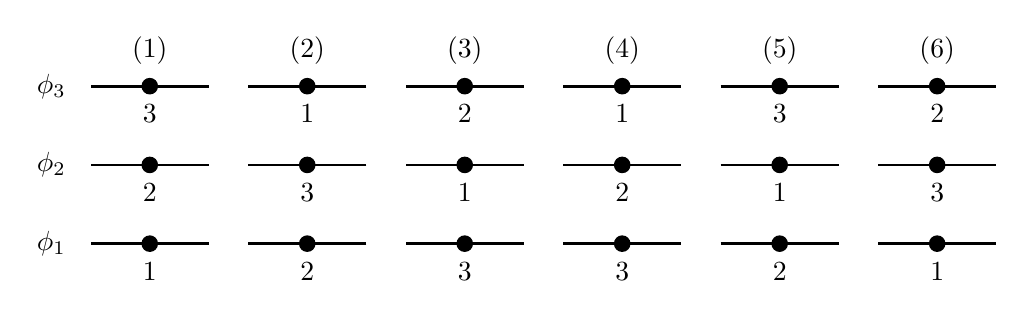
\begin{tikzpicture}
    \node at (-6.25, 2) {$\phi_3$};
    \node at (-6.25, 1) {$\phi_2$};
    \node at (-6.25, 0) {$\phi_1$};

    \node at (-5, 2.45) {(1)};
    \draw[line width=1pt] (-4.25, 2) -- (-5.75, 2);
    \draw[line width=1pt] (-4.25, 1) -- (-5.75, 1);
    \draw[line width=1pt] (-4.25, 0) -- (-5.75, 0);
    \fill (-5, 0)circle(3pt) (-5, 1)circle(3pt) (-5, 2)circle(3pt);
    \node at (-5, -0.35) {$1$};
    \node at (-5,  0.65) {$2$};
    \node at (-5,  1.65) {$3$};

    \node at (-3, 2.45) {(2)};
    \draw[line width=1pt] (-2.25, 2) -- (-3.75, 2);
    \draw[line width=1pt] (-2.25, 1) -- (-3.75, 1);
    \draw[line width=1pt] (-2.25, 0) -- (-3.75, 0);
    \fill (-3, 0)circle(3pt) (-3, 1)circle(3pt) (-3, 2)circle(3pt);
    \node at (-3, -0.35) {$2$};
    \node at (-3,  0.65) {$3$};
    \node at (-3,  1.65) {$1$};

    \node at (-1, 2.45) {(3)};
    \draw[line width=1pt] (-0.25, 2) -- (-1.75, 2);
    \draw[line width=1pt] (-0.25, 1) -- (-1.75, 1);
    \draw[line width=1pt] (-0.25, 0) -- (-1.75, 0);
    \fill (-1, 0)circle(3pt) (-1, 1)circle(3pt) (-1, 2)circle(3pt);
    \node at (-1, -0.35) {$3$};
    \node at (-1,  0.65) {$1$};
    \node at (-1,  1.65) {$2$};

    \node at (1, 2.45) {(4)};
    \draw[line width=1pt] (0.25, 2) -- (1.75, 2);
    \draw[line width=1pt] (0.25, 1) -- (1.75, 1);
    \draw[line width=1pt] (0.25, 0) -- (1.75, 0);
    \fill (1, 0)circle(3pt) (1, 1)circle(3pt) (1, 2)circle(3pt);
    \node at (1, -0.35) {$3$};
    \node at (1,  0.65) {$2$};
    \node at (1,  1.65) {$1$};

    \node at (3, 2.45) {(5)};
    \draw[line width=1pt] (2.25, 2) -- (3.75, 2);
    \draw[line width=1pt] (2.25, 1) -- (3.75, 1);
    \draw[line width=1pt] (2.25, 0) -- (3.75, 0);
    \fill (3, 0)circle(3pt) (3, 1)circle(3pt) (3, 2)circle(3pt);
    \node at (3, -0.35) {$2$};
    \node at (3,  0.65) {$1$};
    \node at (3,  1.65) {$3$};

    \node at (5, 2.45) {(6)};
    \draw[line width=1pt] (4.25, 2) -- (5.75, 2);
    \draw[line width=1pt] (4.25, 1) -- (5.75, 1);
    \draw[line width=1pt] (4.25, 0) -- (5.75, 0);
    \fill (5, 0)circle(3pt) (5, 1)circle(3pt) (5, 2)circle(3pt);
    \node at (5, -0.35) {$1$};
    \node at (5,  0.65) {$3$};
    \node at (5,  1.65) {$2$};
\end{tikzpicture}
	\caption{三粒子填充三条能级的体系集体波函数情况}
	\label{fig:three-body-wv}
\end{figure}

%%%%%%%%%%%%
\paragraph*{平均场的迭代求解}
平均场哈密顿量$H_{mf}$作用到$A$核子的集体波函数$\Psi_0(\bm{r}_1, \bm{r}_2, \cdots, \bm{r}_A)$上可得到原子核的总能量,得到相应的Sch{\"o}dinger方程
\begin{equation}
	H_{mf} \Psi_0 = E \Psi_0
	\label{eq:mf-scho-eq}
\end{equation}
由\cref{eq:mf-hamil},原子核集体波函数分写成单粒子波函数的直乘形式
\begin{equation}
	\Psi_0(\bm{r}_1, \bm{r}_2, \cdots, \bm{r}_A) = \phi_{\alpha_1}(\bm{r}_1) \phi_{\alpha_2}(\bm{r}_2) \cdots \phi_{\alpha_A}(\bm{r}_A)
	\label{def:collect-wv}
\end{equation}
$\phi_{\alpha_{i}}$表示不同能级上的单粒子波函数。

由\cref{eq:mf-hamil,eq:mf-scho-eq,def:collect-wv},平均场下的\textsl{Hartree(-Fock)}方程如下(表示单个粒子的类Sch{\"o}dinger方程):
\begin{equation}\boxed{
    \begin{aligned}
        \frac{-\hbar^{2}}{2m_N} \nabla^{2} \phi_{\alpha}(\bm{r}) + V_{H(F)}\left(
        \{\phi_{i}(\bm{r})\}\right)\phi_{\alpha} = \varepsilon_{\alpha}\phi_{\alpha}(\bm{r}) \\ 
        i = 1, 2, \cdots, A, \quad \alpha = 1, 2, \cdots, \infty
    \end{aligned}
    \label{eq:Hartree-Fock}
}\end{equation}
原子核能量为单粒子能量之和
\begin{equation}
	E = \sum_{i = 1}^{A} \varepsilon_{\alpha_i}
\end{equation}
$\varepsilon_{\alpha_i}$表示第$i$个粒子所在能级对应的能量。

\Cref{eq:Hartree-Fock}与Sch{\"o}dinger方程唯一不同就是势能变成了关于波函数的非线性函数,
\begin{equation*} V(\bm{r}) \Longrightarrow V_{H(F)}(\{\phi_{i}(\bm{r})\})
\end{equation*}
\Cref{eq:Hartree-Fock}为非线性方程组,一般用迭代的方法求解。我们先猜测得到一组试探
波函数$\{\phi_i^0(\bm{r})\}_{i=1}^{A}$,然后我们根据势能与波函数的关系得到初始势场
$V_{H(F)}^{0}$;完成上述步骤后,我们将试探波函数和初始势场带入\cref{eq:Hartree-Fock},
求解得到一组新的波函数$\{\phi_{\alpha}^1(\bm{r})\}_{\alpha=1}^{A}$和本征值$\varepsilon_{\alpha}^{(1)}$,
通过这组新的波函数,我们可以再次生成一个新的势场$V_{H(F)}^{(1)}$;将生成的新势场和新波函数
再次代入式\eqref{eq:Hartree-Fock},可得到更新一组的本征波函数和本征能量。通过比较某次迭代
前后的波函数间的误差小于某一给定值来确定波函数合理
\begin{equation}
    \parallel \phi_{\alpha}^{(n-1)} - \phi_{\alpha}^{(n)} \parallel < \text{preset limit}
    \label{eq:iter-error}
\end{equation}
其中,$\parallel \cdots \parallel$表示波函数的模。

此方法得到的势场一般为中心势场,只适合描述球形核。对于形变核需要进行额外的处理。

\paragraph*{关于平均势场和初始波函数形式的选取}
上述平均场方程中,势能具体形式为\citep[][Eqs. C2.3 and C2.6]{ningpz}
\begin{equation}\boxed{\begin{aligned}
    V_{H}\left( \left\{ \phi_i(\bm{r}) \right\} \right) \phi_j(\bm{r}_j) &= \sum_{i \neq j} \int 
    \phi_i^{\star}(\bm{r}_i^{\prime}) V_{ij}(\bm{r}_i^{\prime}, \bm{r}_j) \phi_{i}(\bm{r}_i^{\prime})
    \,d\bm{r}_i^{\prime}\ \phi_j(\bm{r}_j) \\
	V_{HF}\left( \left\{ \phi_i(\bm{r}) \right\} \right) \phi_j(\bm{r}_j) &= \sum_{i} \int 
    \phi_i^{\star}(\bm{r}_i^{\prime}) V_{ij}(\bm{r}_i^{\prime}, \bm{r}_j) \phi_{i}(\bm{r}_i^{\prime}) \phi_j(\bm{r}_j) - \phi_i^{\star}(\bm{r}_i^{\prime}) V_{ij}(\bm{r}_i^{\prime}, \bm{r}_j) \phi_{i}(\bm{r}_j) \phi_j(\bm{r}_i^{\prime})
    \,d\bm{r}_i^{\prime}  
    \label{eq:mean-field}
\end{aligned}}\end{equation}
为寻找到一组合适的平均场,试探波函数可以选取一组零级近似,如费米气体模型单粒子波函数:
\begin{equation}
    \phi_i = \sqrt{V^{-1}} \exp{(i \bm{k}_i \cdot \bm{r}_i)}
    \label{eq:fermi-gas-eigen}
\end{equation}
其中,$V$表示原子核的体积。对于二体势$V_{ij}$,可以选用Skyrme力(见下式)或其它形式的两体力
\begin{equation}
    V_{skyrme} = \sum_{i<j} v(i, j) + \sum_{i<j<k} v(i, j, k)
    \label{eq:skyrme-forc}
\end{equation}
其中,两体力部分为
\begin{equation}
    \begin{aligned}
        v(1, 2) =& t_0 (1 + x_0 P_{\sigma})\delta(\bm{r}_1 - \bm{r}_2) \\
            & + t_1\left[ \delta(\bm{r}_1 - \bm{r}_2) \bm{k}^{2}
              + \bm{k}^{\prime 2}\delta(\bm{r}_1 - \bm{r}_2)\right] / 2 \\
            & + t_2\bm{k}^{\prime} \cdot \delta(\bm{r}_1 - \bm{r}_2) \bm{k} \\
            & + {\rm i} W_0(\bm{\sigma}_1 + \bm{\sigma}_2)\cdot \left[ 
            \bm{k}^{\prime} \times \delta\left( \bm{r}_1 - \bm{r}_2 \right) \bm{k}\right]
    \end{aligned}
    \label{eq:skyrme-tow-body-forc}
\end{equation}
三体部分为
\begin{equation}
    v(1, 2, 3) = t_3 \delta(\bm{r}_1 - \bm{r}_2) \delta(\bm{r}_2 - \bm{r}_3)
    \label{eq:skyrm-three-body-forc}
\end{equation}
式中,$\bm{k} = \bm{p}/\hbar = (\nabla_{1} - \nabla_{2}) / (2{\rm i})$是向右作用的相对动量
算符,$\bm{k}^{\prime} = \bm{p}/\hbar = (\nabla_{2} - \nabla_{1}) / (2{\rm i})$是向左相对
动量算符;$P_{\sigma} = (1 + \bm{\sigma}_1 \cdot \bm{\sigma}_2) / 2$是自旋交换算符。上式
Skyrme力有6个可调参数$t_0$、$t_1$、$t_2$、$t_3$、$x_0$和$W_0$。

%%%%%%%%%%%%
\paragraph*{唯象势}
一般地,可以选取合适的势场作为固定的原子核集体势场,不需要进行迭代求解,这样选取的势场称为\CJKunderdot{唯象势}。唯象势使对原子核的计算更加简单,但会带来计算上的误差。
常用的两种唯象势
\begin{enumerate}
	\item 三维谐振子势
		\begin{equation}
			v_{ho}(r) = -V_1 + k r^2 = -V_1 + \frac{1}{2} m_N \omega r^2
		\end{equation}
		$V_1$和$k$由实验拟合。
	\item Woods-Saxon势
		\begin{equation}
			v_{ws}(r) = \frac{-V_0}{1 + e^{(r-R)/a}}
		\end{equation}
	一般的取值为
	\begin{equation}
		\begin{aligned}
			R = r_0 A^{\frac{1}{3}} = 1.27  A^{\frac{1}{3}}\ \rm{fm} \quad (nuclear radius) \\
			a = 0.67\ \rm{fm} \quad (surface diffuseness) \\
			V_0 = \left(55 \pm 33 \frac{N - Z}{A}\right) \ \rm{MeV}
		\end{aligned}
	\end{equation}
	质子取$+$,中子取$-$,当不区分核子时取$V_0 = 57\,\rm{MeV}$。
\end{enumerate}


%%%%%%%%%%%%%%%%%%%%%%%%%%%%%
\section{Woods-Saxon波函数}
基于以上给出的唯象Woods-Saxon势,并结合库伦势和自旋-轨道耦合作用,可以对原子核的类Sch{\"o}dinger方程进行数值求解,并将波函数在谐振子基下展开。

\paragraph*{单核子哈密顿量}
单核子薛定谔方程中的哈密顿量为:
\begin{equation}
	\begin{aligned}
		h =&\, \frac{-\hbar^2}{2 m_{N}} \nabla^2 + v(r) + v_{LS}(r) \bm{L}\cdot \bm{S}	\\
		=&\, \frac{-\hbar^2}{2 m_{N}}\left(\nabla^2_{r} - \frac{\bm{L}^2/\hbar^2}{r^2}\right) + v_{WS}(r) + v_{C}(r) + v_{LS}(r)\boldsymbol{L\cdot S}
	\end{aligned}
\end{equation} 
其中,径向偏分取一般形式
\begin{equation}
	\nabla^2_{r} \equiv \frac{1}{r^2} \frac{d}{dr} \left(r^2 \frac{d}{dr}\right)
\end{equation}
表示径向动能;括号中的第二项为核子“离心势能”项,它使系统总能量降低(所谓“向心力”是由势场提供的,核子的转动越大,它就有更大的能量脱离原子核,也就是离心势);$v_{WS}$是唯象Woods-Saxon势;$v_{C}(r)$为库伦势,只表示质子间的相互作用,若为中子,该项取0,原子核半径内取均匀带电的球静态库伦势,可得方程如下
\begin{equation}
	v_{C} = \frac{Ze^2}{4\pi\epsilon_0} \left\{
		\begin{aligned}
			&\frac{3 - (r/R)^2}{2R}, \quad & r\leqslant  R \\
			&\frac{1}{r}, \quad            & r > R  
		\end{aligned}
	\right.
\end{equation}
自旋-轨道耦合项系数为
\begin{equation}
	v_{LS}(r) = v_{LS}^{(0)} \left(\frac{r_0}{\hbar}\right)^2 \frac{1}{r} \left[\frac{d}{dr} \frac{1}{1 + e^{(r-R)/a}}\right]
	\label{eq:spin-orbit-der-term}
\end{equation}
中括号的偏分表示不作用到波函数上,并且这个偏分将使自旋-轨道耦合的峰位处于原子核表面区域。
\begin{example}[自旋-轨道耦合偏分项]
	假设原子核质量数$A = 100$,则对应的半径为$R = 1.27 \times 100^{\nicefrac{1}{3}} \approx 5.895\, \rm{fm}$,则\Cref{eq:spin-orbit-der-term}中的偏分项$f = \frac{d}{dr} \frac{1}{1 + e^{(r-5.895)/0.67}}$的图像如\Cref{fig:spin-orbit-der-term}
	\begin{figure}[htbp]
		\centering
		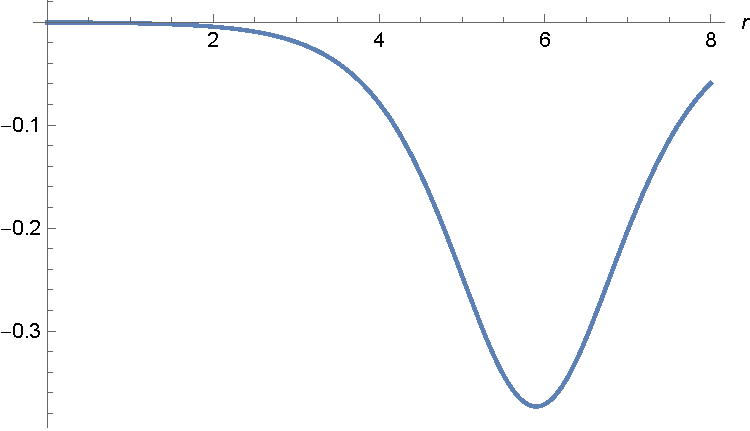
\includegraphics[scale=0.6]{figure/nuclear/spin-orbit-der.pdf}
		\caption{自旋轨道耦合偏分项}
		\label{fig:spin-orbit-der-term}
	\end{figure}
	可见,在原子核表面区域确实存在一个峰值,这表明原子核表面处自旋轨道耦合作用最强。
\end{example}
自旋-轨道耦合中的半径依赖通常可以用一个常数取代,我们取强度
\begin{equation}
	v_{LS}^{(0)} = 0.44 V_0
\end{equation}

\paragraph*{波函数用谐振子基展开}
三维谐振子波函数构成一组正交基,Woods-Saxon势下的原子核单粒子波函数可用这组谐振子基进行展开:
\begin{equation}
	f_{nlj}(r) = \sum_{\nu} A_{\nu}^{(nlj)} g_{\nu l}(r), \quad \sum_{\nu} [A_{\nu}^{(nlj)}]^2 = 1
\end{equation}
这样得到的核单核子波函数的细节见\Cref{sec:mat-diag}。

\paragraph*{Woods-Saxon哈密顿量的对角化}
得到球谐振子波函数后,可将这些波函数作为基矢展开构成Woods-Saxon势下的原子核波函数。谐振子展开的Woods-Saxon径向哈密顿量矩阵元为
\begin{equation}
    \begin{aligned}
		\langle \nu^{\prime} | h_{lj}(r) | \nu\rangle =&\int_{0}^{\infty} r^2 \,dr g_{\nu^{\prime} l}^{\ast}(r) g_{\nu l}(r) \left[ \frac{\hbar^2}{2m_N} \left(\frac{4n + 2l + 3}{b^2} - \frac{r^2}{b^4}\right) \right. \\
		&+ \left. v_{WS}(r) + v_{C}(r) + \frac{1}{2}\left[j(j+1) - l(l+1) - \frac{3}{4}\hbar^2 v_{LS}(r)\right] \right]
    \end{aligned}
\end{equation}
这样,整个矩阵就可以写成如下形式
\begin{equation}
	\begin{bmatrix}
		\langle 0 | h_{lj}(r) | 0 \rangle & \langle 0 | h_{lj}(r) | 1 \rangle & \cdots	& \cdots	\\
		\langle 1 | h_{lj}(r) | 0 \rangle & \langle 1 | h_{lj}(r) | 1 \rangle & \cdots	& \cdots	\\
		\vdots	&	\vdots	& \ddots & \vdots \\
		\cdots	&	\cdots	& \cdots & \ddots
	\end{bmatrix}
\end{equation}
这样,当我们对角化该矩阵后就可以知道此径向哈密顿量本征能量,利用\Cref{eq:expand-coeff}或\Cref{eq:expand-basis-matform}就可以知道对应谐振子基上的系数$A_{\nu}^{(nlj)}$并构建相应的Woods-Saxon波函数。

相应的计算结果可参看J. Suhonen编纂的核物理书《\textit{From Nucleons to Nucleus Concepts of Microscopic Nuclear Theory}》中的Tab. 3.1 - 3.4以及Fig. 3.4。

\paragraph*{需要注意的点}
在径向薛定谔方程中,由于$\nicefrac{l(l+1)}{r^2}$的存在,当$l>0$时该项对正能量的那部分区域的作用相当与叠加了一个“离心势垒”,并在该势垒内产生准定态(quasi-stationary)的、长寿命的单粒子态。因此\CJKunderline{一些高能态具有正的能量,但它们依然为离散态而非连续态。}

离心位垒的高度为
\begin{equation}
	v_{cf}(R) = \frac{\hbar}{2m_N} \frac{l(l+1)}{R^2} \approx 13.2 A^{-2/3} l(l+1)\, \rm{MeV}
\end{equation}

自旋轨道耦合产生的能级劈裂对应的能量差为
\begin{align}
	\Delta_{nl}^{ls} = \varepsilon_{nlj_{-}} - \varepsilon_{nlj_{+}} \approx -(l + \frac{1}{2})\hbar^2 C_{nl} \\
	C_{nl} = \frac{C_{nlj_{+}} + C_{nlj_{-}}}{2},
	\quad
	C_{nlj} = \int_{0}^{\infty} r^2\, dr\, f_{nlj}^2(r) v_{ls}(r)
\end{align}

%%%%%%%%%%%%%
\section{多核子组态}
\paragraph*{“坐标表象”}
同时描述自旋为$\nicefrac{1}{2}$的旋子的坐标空间$\bm{r}$及自旋空间$\bm{\chi}$的表象,简记为$\bm{x}$。

\paragraph*{多核子组态}
单粒子态和单粒子能量是原子核壳模型的基础。对单粒子态做如下约定:
\begin{equation}\boxed{
	\ket{\phi_{\alpha}} \equiv \ket{\alpha} \equiv \ket{am_{\alpha}}, \quad a \equiv n_{a} l_{a} j_{a} \label{eq:sgl-part-stat}
}\end{equation}
其中,$l_a$和$n_a$是$a$轨道的轨道量子数和总角动量量子数,$n_a$为主量子数,$m_{\alpha}$则是$j_a$在$z$轴的第三分量量子数。



\bibliographystyle{modified-apsrev4-2}
\bibliography{reference}